\documentclass[letterpaper,12pt]{article}

%TeXcount at http://app.uio.no/ifi/texcount/online.php

%\setlength{\parindent}{0in}
%\usepackage{fullpage} 
\usepackage{amsmath}
\usepackage{amssymb}
\usepackage{enumerate}
\usepackage{graphicx}
\usepackage[table]{xcolor}
\usepackage{dcolumn}
\oddsidemargin 0.0in
\textwidth 6.5in
\newcolumntype{.}{D{.}{.}{-1}}
\newcommand*{\myalign}[2]{\multicolumn{1}{#1}{#2}}

%opening
\title{Evolution and Military Adoption \\ of Commercial Smart Phones}
\author{Steve Mazza}
\date{September 3, 2012}

\begin{document}
\maketitle

\begin{abstract}
The evolution of commercial smart phones and subsequent early adoption by Department of Defense (DoD) is better understood by first looking at the technology.  After establishing a working description, we look at some of the market drivers that have shaped the evolution and high growth of the devices.  For a better understanding of the direction they are headed, we look at the technology and forces that came together to enable current smart phones.  We wrap up by discussing the different variants, rates of adoption and permutation, and provide a brief forecast for the ten year horizon contrasting civilian and military use.
\end{abstract}

% Make 2 parts per section: first about the technology in general and second about the Army's use of it.
\section*{Technology Description}
% Describe the technology and include pictures, drawings, or other illustrations as appropriate.
Smart phones are the result of the intersection of several mature and emerging consumer technologies including cellular, WiFi, Bluetooth, and near field communications (NFC) tightly coupled with various sensors such as accelerometer, global positioning system (GPS), compass, proximity, and touch.  The smart phone revolution started in early 2003 with the introduction of the BlackBerry Quark\footnote{Wikipedia, \emph{List of BlackBerry Products}, http://en.wikipedia.org/wiki/List\_of\_BlackBerry\_products (as of \today).}.  Fueled by consumer demand, Microsoft and Palm entered the market.  But it wasn't until Apple introduced the iPhone that the revolution fully took hold.  No longer just the tools of the business elite, now these devices were actively marketed to the average consumer -- equally at home in the boardroom and in your kid's backpack.

\section*{Technological Need}
% What are the needs the technology fulfills � think back to SE3100 when you did a capability needs analysis.  Define and/or model as appropriate the needs (wants) the technology fulfills.  What functions does the technology provide?  How does it fit into its environment?
More and more, our lives put us on the go.  In a consumer driven market, manufacturers respond to the needs of our lifestyles.  Whether for work or personal use, our smart phones span the distance from home, to the gym, to work, and are even with us on our commute time in between.  In the Army's case, warfighters' needs are not all that different and smart phones are finding a niche in stateside training commands, permanent CONUS duty stations, and at different echelons in theater from Division all the way down to the dismounted soldier on patrol.  

Key enablers of these devices both for military and for civilian use are the reduction in size, weight, power, and cost compared with carrying similar previous generation devices.  Prior to the introduction of the smart phone, the end user would need an MP3 player, a hand held GPS, a cellular phone, and a laptop in order to get the same functionality; the size, weight, power, and cost of which were all prohibitive.  Today, all of this functionality slips neatly into your pocket and costs less than \$500.00.  That cost is a strong driver of both civilian and DoD market penetration and adoption.

Furthermore, many consumers have chosen to forgo a traditional land line, trading phone and long distance charges for cellular and data charges.

\section*{Evolution of the Technology}
% How has the technology evolved over its history?  Research when the technology was first introduced, how it was introduced, and its major milestones over the technology�s lifetime.
Started by Blackberry and fueled by unrelenting consumer demand, the history of the smart phone market has been marked by the introduction of several disruptive technologies.  As early as 1983, Motorola began commercial marketing of the DynaTAC 8000X.  

\begin{center}
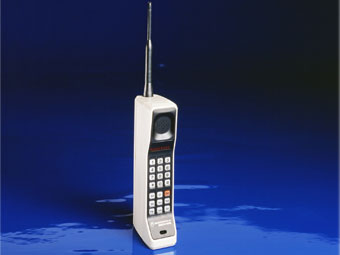
\includegraphics[scale=0.7]{images/dynaTac8000}
\end{center}

Cell phones continued to progress at a steady albeit slow pace through the introduction of the Palm Pilot in 1996 which, while it contained no cellular capability, brought together many other features of the personal organizer.  Interestingly, the pre-Jobs Apple Newton introduced in February, 1998, went almost completely unnoticed by consumers.  

\begin{center}
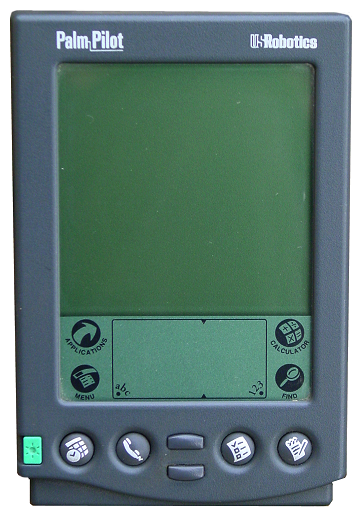
\includegraphics[scale=0.3]{images/Palmpilot5000}
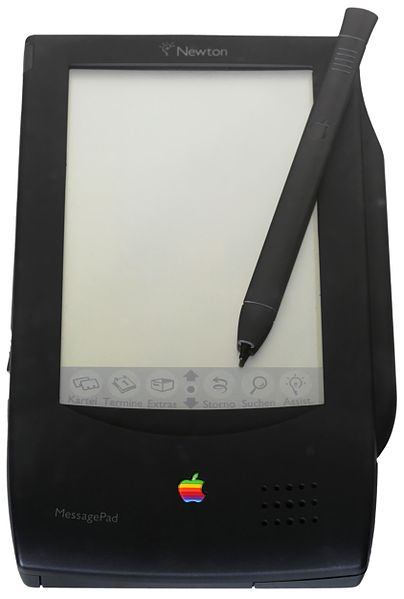
\includegraphics[scale=0.3]{images/Apple_Newton}
\end{center}

It wasn't until the introduction of the Blackberry Quark by Research In Motion (RIM) that consumer demand for an integrated cell phone and personal digital assistant (PDA) really caught hold.  RIM's rise to the top would prove to be as quick as its reign was short-lived.  Apple's introduction of the iPhone in early 2007 marked the greatest advance in this consumer technology and took the market by storm. 

\begin{center}
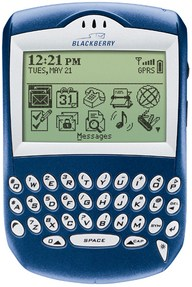
\includegraphics[scale=0.8]{images/blackberry_6200}
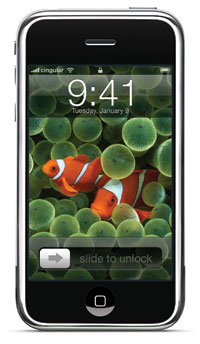
\includegraphics[scale=0.6]{images/apple-iphone}
\end{center}

Shortly thereafter, Google released the first commercial version of the Android operating system in September, 2008, code named \emph{Astro}.  Android continues to provide significant market pressure fueling innovation and lowering the barrier to market penetration.  By the end of 2010, Android became the world's leading smart phone platform\footnote{Wikipedia, \emph{Android (operating system)}, http://en.wikipedia.org/wiki/Android\_(operating\_system), (as of \today).}.

\section*{Technologically Enabling Advances}
% What technical advances in related or component technologies enable this technology?  What knowledge is associated with the development of the technology? (e.g., mechanical knowledge, nuclear, �)
Smart phone technology is really a system of systems, bringing together a cadre of sensors, cellular, and WiFi capability (plus more recently near field communications, or NFC) under an integrated and unified user interface which is facilitated by touch screen capability.  The technology enabling advances have principally been increases battery life, reductions in power draw, and the ability to produce inexpensive, high resolution capacitive touch screens.

As GPS plays such a prominent role in current smart phone technology, enabling location aware services for civilian and military users alike, the 1996 policy directive issued under then president Bill Clinton that opened the GPS signal up to civilian use was a critical enabling technology.

It is arguable that Apple's introduction of the iPod in November, 2001\footnote{Wikipedia, \emph{iPod}, http://en.wikipedia.org/wiki/IPod, (as of \today).}, did much to fuel the commercial smart phone industry by identifying an opportunity and packaging an affordable, portable, and attractive solution thus creating a new consumer market.  It paved the way for consumers to expect more diverse capabilities from their portable electronic devices and allowed industry to see beyond the previous limitation of the traditional cellular phone.

Given the current climate of constrained defense budgets as well as consumer belt tightening, we cannot completely decouple the technological advances from the economic enablers as we attempt to understand the rapid growth of the commercial smart phone market.  As well as the important technological leaps forward mentioned above, it is an economy of scale in manufacturing and marketing that have provided a price point that is just within the threshold for consumer spending.  Without this important market force, amortizing the significant research and development spending in the private sector by companies like Apple, Nokia, Samsung, HTC, RIM, and others, the unit cost would be significantly higher thus increasing the barrier to adoption for military use.

\section*{Variants of the Technology}
% Are there variants of the same technology?  If so, what are the differences/similarities of those variants?  (e.g., automobile technology, there are variants in engine type, transmission, etc.).  Variants indicate either different needs, different prioritization of needs, or different solution approaches to the same problem.
Today we see a highly fragmented smart phone market and while this is representative of relatively minor differences (mostly based on implementation of the technologies), there is a larger landscape of related devices that covers a more diverse technological landscape.  As phones grow larger, the line between the smart phone and tablet continues to blur.  The iPad still dominates the tablet market but Android continues to gain market share mostly due to their attractive price point.

Other variants of smart phone technology include the Google and Apple TV set top boxes.  These are tightly integrated, Internet connected devices that aggregate information and games as well as traditional broadcast content onto the television.  While not usually containing cellular capability, these devices run variants of the same operating systems found on commercial smart phones.  The Google Glasses project represents another offshoot extension to smart phone technology and promised to provide a hands-free wearable alternative to present offerings.

Ubuntu, a division of Canonical, Ltd., is working on a version of its Linux operating system (the kernel of which forms the basis for Android) that will tightly integrate with Android and will move the smart phone and desktop closer together.

While the military works toward adoption of smaller, lighter, faster, cheaper commercial devices, they still make use of ruggedized tablets and PDAs.  These are bulky and hindered by short battery life and, consequently, are not usually well received by today's digitally aware warfighters.

\section*{Technology Diffusion}
% Explain the mechanisms and timing of how the technology diffused through the market, military, or society?  How long did it take to be adopted?
The military has been cautious in its approach to the adoption of commercial smart phone technology.  Hamstrung by an acquisition process that is not well suited to fielding fast moving technology, the military communities have largely relegated the use of commercial smart phones to trials and limited fielding.

The much more agile civilian consumer market has responded more quickly and provided almost limitless demand for continued development.  While cell phone market growth was steady, the market cracked wide open following the introduction of Apple's iPhone in 2007.

Ironically, it is the same demographic that comprises the typical warfighter that also tends to be among the early adopters of smart phone technology.

\section*{Growth Rate}
% What has been the growth rate of the technology?  Define appropriate measures of effectiveness and/or performance and determine its growth rate.  For example, for automobiles you could look at mpg, average service life, reliability, and other relevant measures.
Smart phones have continued to replace traditional cell phones, sometimes called \emph{feature phones}, at an increasing rate.  

\begin{center}
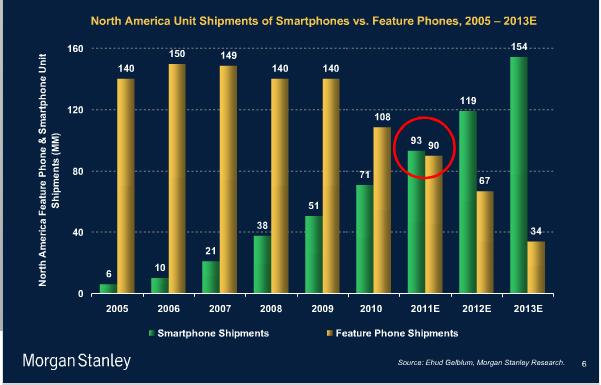
\includegraphics[scale=0.5]{images/growthRate}
\end{center} 

The principal measure of effectiveness describing this growth is connectivity. As cellular infrastructure becomes more ubiquitous, fast, and reliable, the applications available to the smart phone that allow us to connect to people and services around us continues to be the compelling force in both civilian and military markets.  While \emph{apps} are what consumers often focus on, it is the connectivity that they facilitate that ultimately drives growth.

\section*{Forecast}
% Forecast likely scenarios of where the technology will be 10 � 20 years from today; and/or create a technology roadmap of where the main stakeholders would likely want the technology to be.
Given that the smart phone market is less than ten years old, it would be impractical to try and predict ten to twenty years out.  But do not despair\dots\ the science fantasy future is much closer at hand.  Within ten years the term \emph{smart phone} will no longer be in use.  I will, however, continue to use it here for the sake of continuity.

\subsection*{Intelligent Agents}
Our phones already provide us with \emph{location aware} information, helping us to make informed decisions about which errands to run, where to eat, and even which friends are nearby.  But the analysis of our surroundings will continue to progress to the point where we will have meaningful information about our choices, actions, and how to organize our day.  Data regarding out intents will be factored into information about our habits, schedule, and the people and resources around us.  This \emph{intelligent agent} technology will streamline our decision making, help us to be productive (vice distracted), and help us make the most of our free time.  The effect of intelligent agents will be highly targeted and relevant data.  It will help us to cut through the clutter (information overload) that we often face today.

\subsection*{Extreme Connectivity}
Today Bluetooth allows us to connect seamlessly to peripherals like headsets and speakers and facilitates integration into dedicated environments such as our automobiles.  The connectivity from our personal devices like smart phones will, however, become almost ubiquitous, connecting us to most elements in our home, school, and work.  No longer will we be required to set our alarm clock; our smart phone will provide an analysis of our day and give us sufficient time to prepare ourselves.  The surface of our nightstand may provide an active display (e.g., display clock and weather data) and touch surface that allows us to interact directly with our smart phone (e.g., retrieve calendar data).

Similarly, at work and at school collaboration will be facilitated by our smart phones but will likely be principally performed using highly connected peripherals.  The analog of the white board will be an interactive touch surface capable of connecting to and interacting with multiple smart phones simultaneously.

Similar to how the interfaces to smart phones have become virtualized through software, the dashboards on our automobiles will become highly adaptable extensions to our devices.  For a glimpse at this vision of the future, see ``A Day Made of Glass 2" produced by Dow Corning (http://www.youtube.com/watch?v=Sc8lzavmXOk\&feature=related).

\subsection*{Physical Connection}
Computational horsepower will continue to increase per Moore's Law.  This will allow smart phones to assume a greater role in processing and providing information.  The mechanism of providing information will continue to evolve closer and closer to our physiology.  Present day vibrations will pale in comparison to integrated heads up displays, wearable devices no larger or more conspicuous than contact lenses.

Similarly, touch surfaces will provide responsive tactile feedback (resistance) capable of accurately simulating the sensation of touching a physical object (e.g., the softness of a kitten or the roughness of sandpaper).  This immersive experience will evolve into an unobtrusive, thin, wearable ``glove" that enhances our interaction with the world around us; a new form of augmented reality.

\subsection*{Military Application}
Warfighters will benefit from all of these advances and will be provided with the exact situational awareness necessary in a context sensitive manner.  Future smart phone technology along with ubiquitous connectivity will ensure that the right information is delivered to the right warfighter at the right time every time.

Warfighters will no longer need to stop what they are doing and bury their heads in a small display.  Interaction with the smart phone will be non-disruptive and non-distracting.  Integration of the smart phone into the warfighter's mission will be completely seamless.

The smart phone has a bright future both in civilian and DoD markets.  It's present demonstration of near limitless growth should continue not just with the pace of computational increases but also with increased connectivity and bandwidth.  Connectivity to new and emerging devices around us will drive consumer demand and will spur military application.  In ten years we won't likely be calling them smart phones (nor are we likely to even recognize them from a form factor standpoint) but highly capable, highly connected devices will continue to evolve as  the cornerstones of our daily routines.

\end{document}